%%%%%%%%%%%%%%%%%%%%%%%%%%%%%%%%%%%%%%%%%%---Appendix
\appendix
%\renewcommand\thefigure{\thechapter.\arabic{figure}}  

\chapter{Supporting Figures}
%\paragraph{Posterior Samples and Summary statistics}
%\setcounter{figure}{0}

\begin{comment}
\begin{table}
\centering
\label{tab:hatp44_summary}
\begin{tabular}{lll}
\hline
d && \\
\hline
\end{tabular}
\end{table}
\end{comment}

%Note that the joint posterior distribution directly show correlations among variables. We confirm that indeed no such correlations exist between limb darkening parameters $q_1$ and $q_2$ as shown by their posterior distributions

\begin{figure}
\centering
\begin{subfigure}{.5\textwidth}
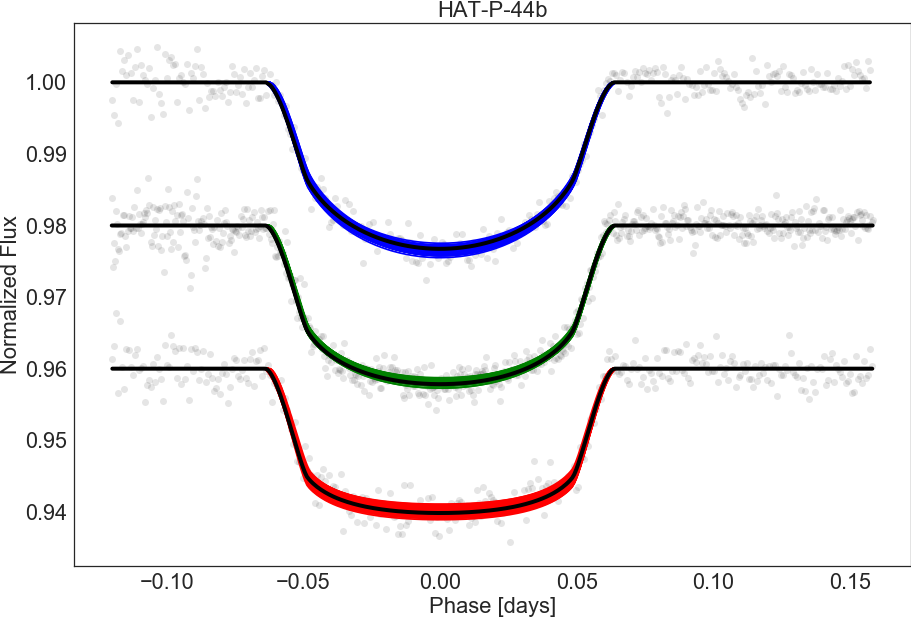
\includegraphics[width=7cm]{hatp44/1000_posterior_samples.png}
\caption{Full best-fit transit models.}
\end{subfigure}%
\begin{subfigure}{.5\textwidth}
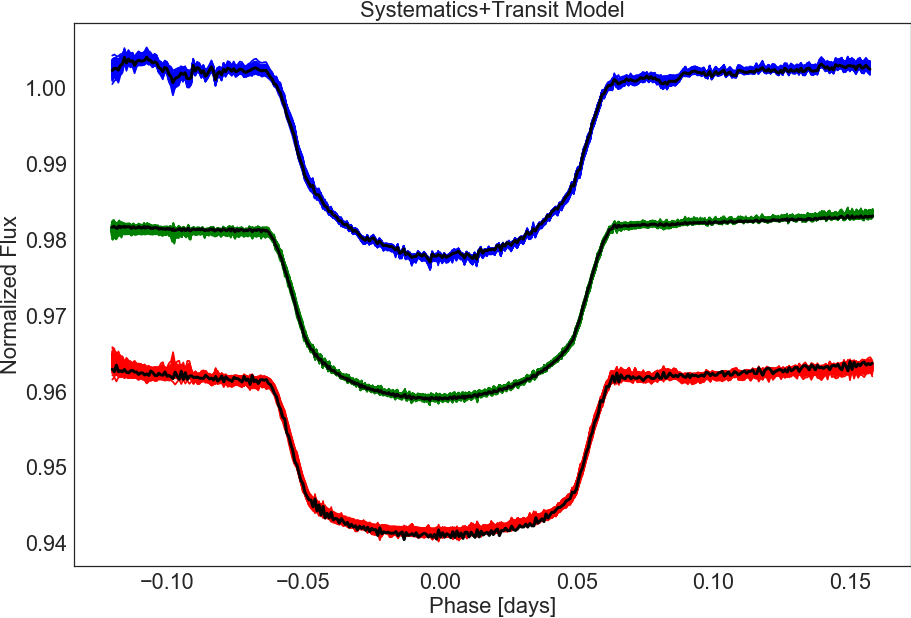
\includegraphics[width=7cm]{hatp44/transit_with_sys.png}
\caption{Full best-fit transit+systematics models.}
\end{subfigure}
\caption{(a) HAT-P-44b's best-fit transit models (black line) superposed with the systematics-corrected data (grey points). The colored lines are 1000 random samples that qualitatively show that the posterior distributions are sufficiently converged. The blue, green, and red correspond to g-,r-,and z-bands respectively. (b) Same as in (a) but with added systematics model.}
\label{fig:hatp44_samples}
\end{figure}

\begin{figure}
\centering
\begin{subfigure}{.5\textwidth}
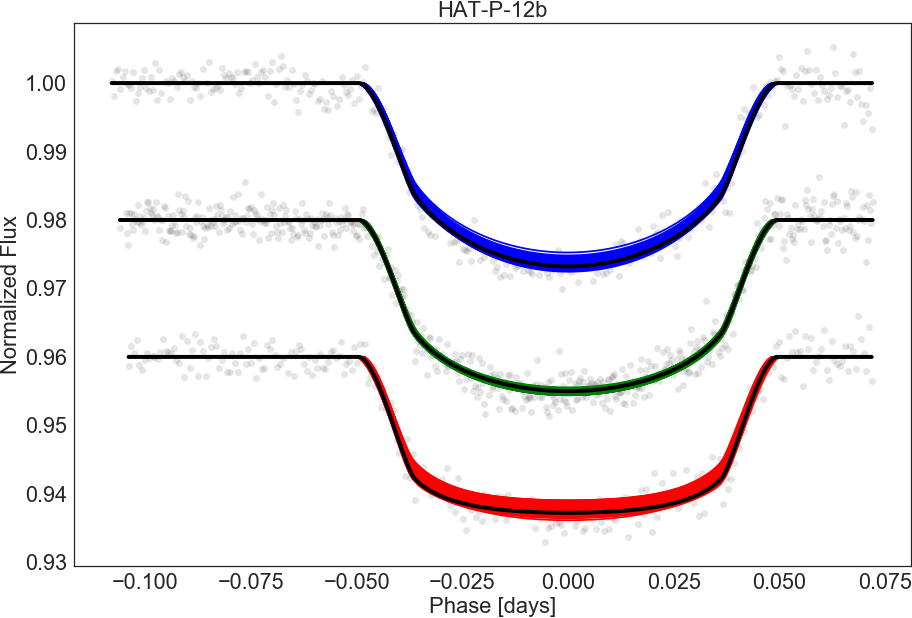
\includegraphics[width=7cm]{hatp12/1000_posterior_samples.png}
\caption{Full best-fit transit models.}
\end{subfigure}%
\begin{subfigure}{.5\textwidth}
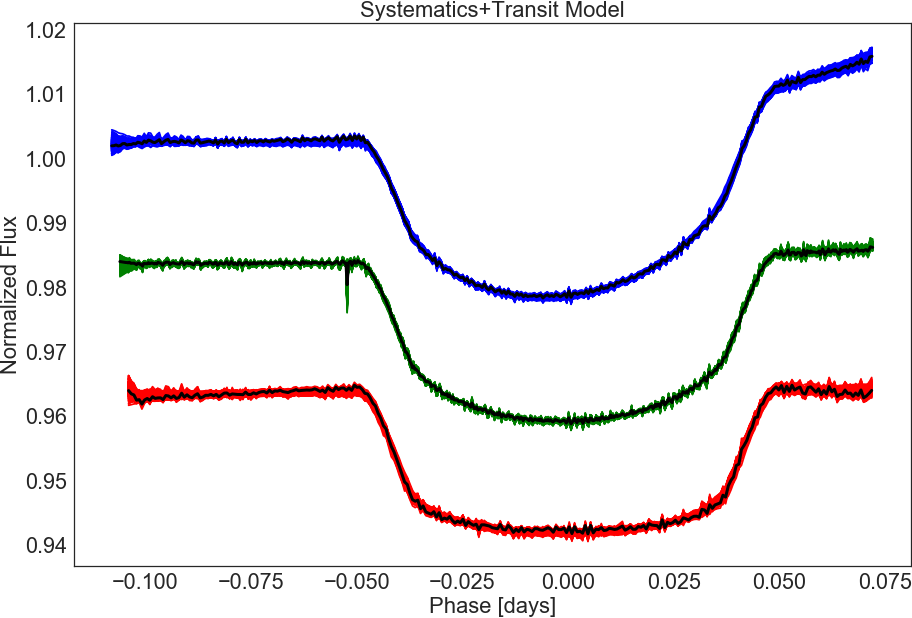
\includegraphics[width=7cm]{hatp12/transit_with_sys.png}
\caption{Full best-fit transit+systematics models.}
\end{subfigure}
\caption{Same as Fig.~\ref{fig:hatp44_samples} but for HAT-P-12b.}
\label{fig:hatp12_samples}
\end{figure}

\begin{figure}
\centering
\begin{subfigure}{.5\textwidth}
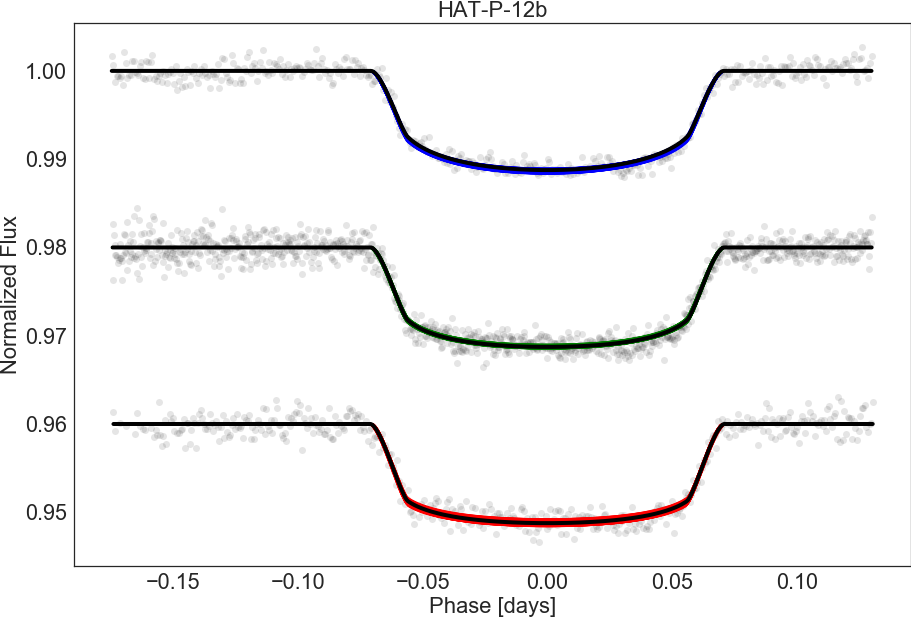
\includegraphics[width=7cm]{wasp21/1000_posterior_samples.png}
\caption{Full best-fit transit models.}
\end{subfigure}%
\begin{subfigure}{.5\textwidth}
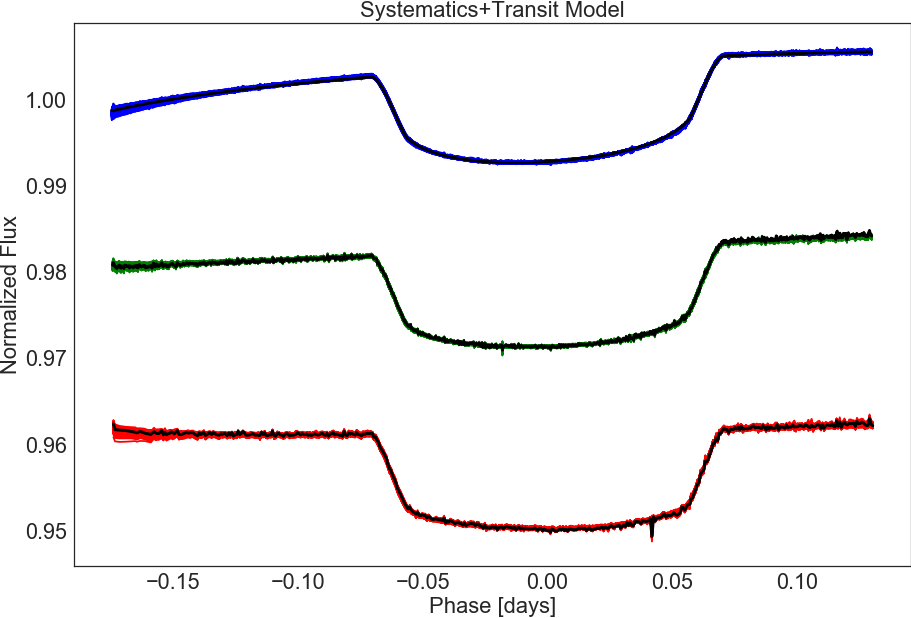
\includegraphics[width=7cm]{wasp21/transit_with_sys.png}
\caption{Full best-fit transit+systematics models.}
\end{subfigure}
\caption{Same as Fig.~\ref{fig:hatp44_samples} but for WASP-21b.}
\label{fig:wasp21_samples}
\end{figure}


%\paragraph{MuSCAT filter transmission curves}
\begin{figure}
\centering
	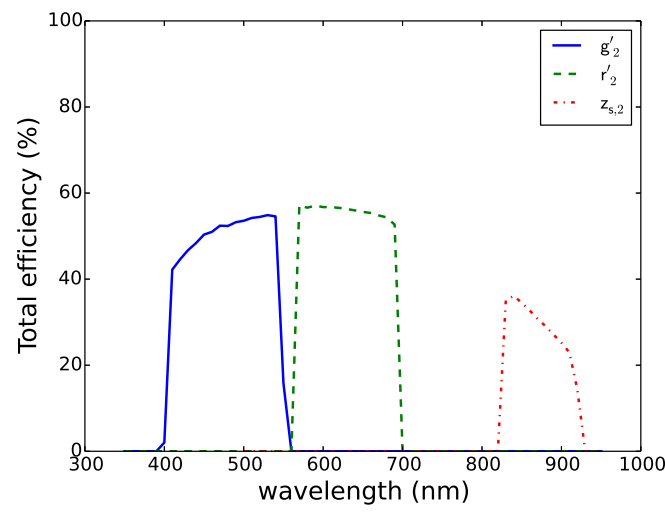
\includegraphics[width=10cm]{figures/MuSCAT_efficiency.png}
    \caption{Transmission curves of OAO/MuSCAT g', r', and z$_{s,2}$ filters. Each curves are integrated to determine the central wavelengths used in plotting the transmission spectrum and calculations.
    }\label{fig:filter_transmission}
\end{figure}

\begin{figure}
\centering
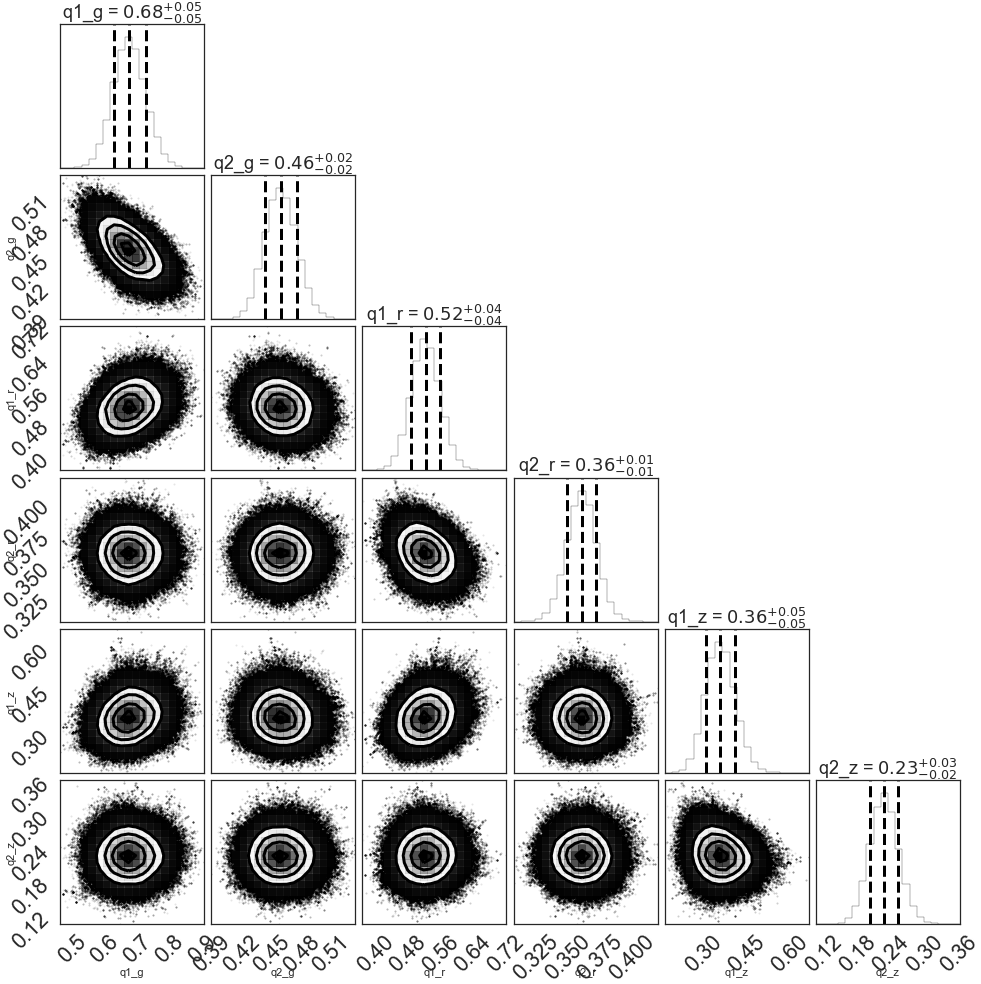
\includegraphics[width=7cm]{hatp44/limbdark_q1q2.png}
\caption{Corner plot of limb darkening coefficients showing joint posterior distributions along off-diagonal and marginalized distributions along the diagonal. As expected, there are no apparent correlations between limb darkening coefficients as shown by the joint plot.}
\label{fig:hatp44_q1q2}
\end{figure}

\begin{figure}
\centering
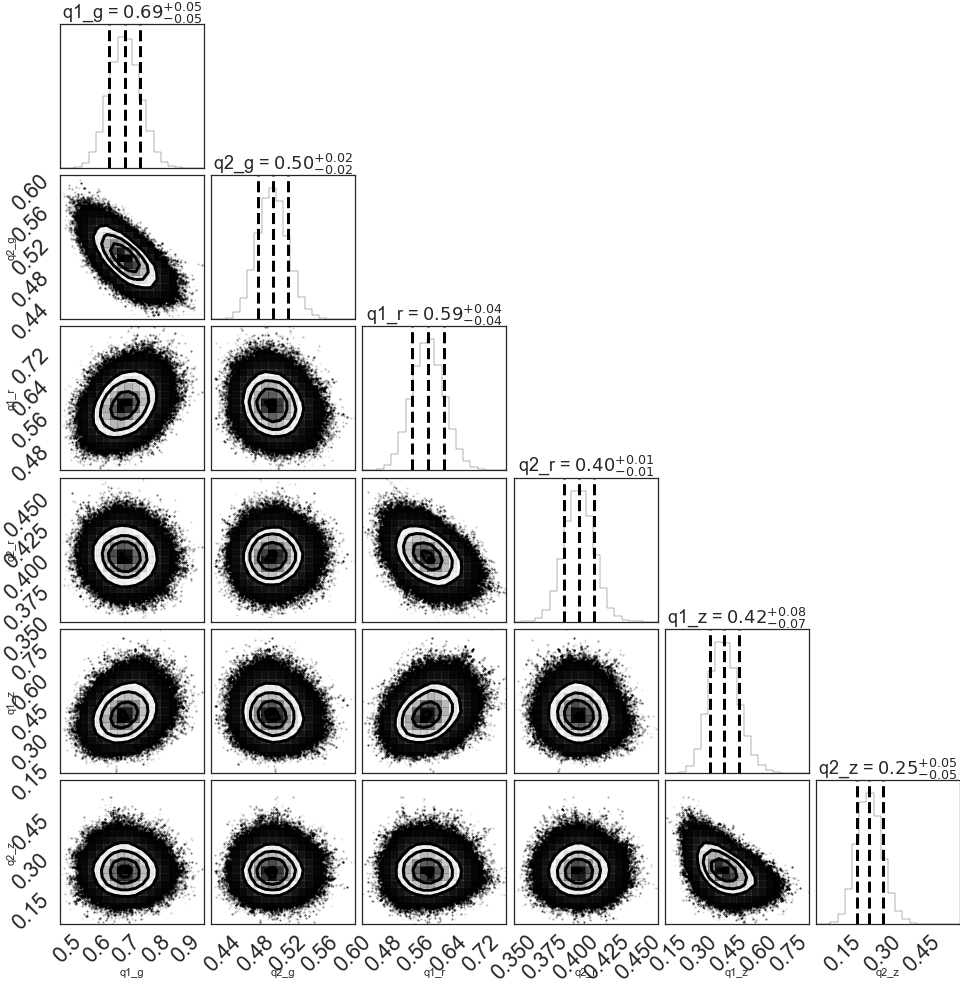
\includegraphics[width=7cm]{hatp12/limbdark_q1q2.png}
\caption{Same as Fig.~\ref{fig:hatp44_q1q2} but for HAT-P-12b.}
\label{fig:hatp12_q1q2}
\end{figure}


\begin{figure}
\centering
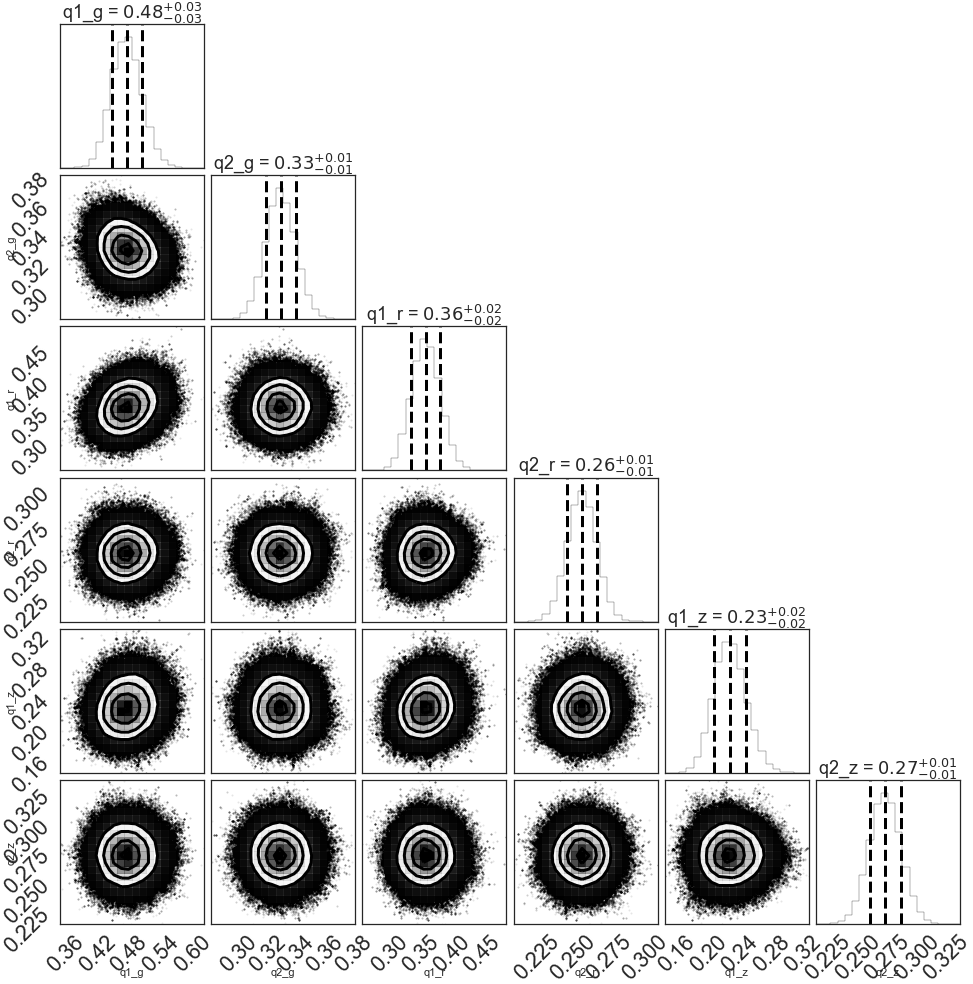
\includegraphics[width=7cm]{wasp21/limbdark_q1q2.png}
\caption{Same as Fig.~\ref{fig:hatp44_q1q2} but for WASP-21b.}
\label{fig:wasp21_q1q2}
\end{figure}

\begin{comment}
%\paragraph{Limb darkening}
%\setcounter{figure}{0}
\begin{figure}
\centering
\includegraphics[width=7cm]{figures/limbdark_blackbodies.png}
\caption{The upper black body corresponds to the solar disk (hotter) and the lower corresponds to the limb (cooler). As we go towards longer wavelengths (red), the ratio of the intensities (area bounded by each bandpasses) approaches 1, i.e. limb darkening effect is negligible in the infrared and more pronoounced in the optical. Thus, we expect to see the shape of z-band flatter than g-band.}
\label{fig:bb}
\end{figure}


\begin{figure}
\centering
\includegraphics[width=7cm]{figures/q_to_u.png}
\caption{Transformation of limb darkening coefficients between $q$- (blue) and $u$-space (red). This transformation constrains our sampling algorithm to explore only physically allowed limb-darkening coefficients, $u$, used to evaluate the Mandel-Agol model (See $\S$\ref{sec:transitmodel}).}
\label{fig:q_to_u}
\end{figure}
\end{comment}

\begin{comment}
\chapter{Model Selection}
We used the Bayes factor to select between competing models. The Bayesian evidence, $Z$, is defined by
\begin{equation}
Z=P(D|M)=\int d\theta P(\theta|M)P(D|\theta,M) 
\end{equation}
where $P(D|M)$ is the probability of observing the data $D$ given model $M$, marginalized over the model parameters $\theta$. The Bayes factor comparing the posterior probabilities for Models $M_1$ and $M_2$ given the data $D$ is defined by: 
\begin{equation}
 K_{1,2}=\frac{P(M_1|D)}{P(M_2|D}=\frac{P(M_1)P(D|M_1)}{P(M_2)P(D|M_2)}
\end{equation}
where P(M) is the prior probability for model $M$. Assuming equal priors for the different models tested, the Bayes factor is then equal to the evidence ratio:
\begin{equation}
 K_{1,2}=\frac{Z_1}{Z_2}
\end{equation}
If $ K_{1,2} > 1$, then $M_1$ is favored over model $M_2$.

In practice, $Z$ is difficult to determine as it requires integrating a complicated function over a high-dimensional space (e.g., Ferroz et al 2009). %https://arxiv.org/pdf/0809.3437.pdf
On the other hand, Weinberg et al. (2013) suggested a simple and relatively accurate method for estimating Z directly from the results of an MCMC simulation. 
\end{comment}